\documentclass[11pt]{article}
\usepackage[reqno]{amsmath}
\usepackage{amssymb}
\usepackage{epsf}
\usepackage{epsfig}
\usepackage{rotate}
\usepackage{hyperref}
\newcommand{\ol}{\overline}
\newcommand{\ul}{\underline}
\newcommand{\vb}{\verbatim}
\newcommand{\bi}{\begin{itemize}}
\newcommand{\ei}{\end{itemize}}
\newcommand{\be}{\begin{enumerate}}
\newcommand{\ee}{\end{enumerate}}
\newcommand{\noi}{\noindent}
\newcommand{\ro}{{\bf R}^1 }
\newcommand{\rn}{{\bf R}^n }
\newcommand{\lra}{\Longrightarrow}
\newcommand{\qlq}{\quad\lra\quad}
\newcommand{\bul}{\bullet}
\newcommand{\llim}{\lim\limits}
\newcommand{\xc}{_{x\to c}}
\newcommand{\nin}{_{n\to\infty}}
\newcommand{\pb}{\parbox{1in}}
\newcommand{\pbof}{\parbox[t]{1.5in}}
\newcommand{\pbt}{\parbox[t]{2in}}
\newcommand{\pbff}{\parbox[t]{4in}}
\newcommand{\rot}{\rotate[r]}
\newcommand{\ep}{\epsffile}
\newcommand{\eps}{\epsilon}
\newcommand{\beqa}{\begin{eqnarray}}
\newcommand{\eeqa}{\end{eqnarray}}
\newcommand{\non}{\nonumber}
\newcommand{\di}{D^{-1}}
\newcommand{\lint}{\int\limits}
\newcommand{\bmat}{\begin{matrix}}
\newcommand{\emat}{\end{matrix}}
\newcommand{\bal}{\begin{align}}
\newcommand{\eal}{\end{align}}
\setcounter{MaxMatrixCols}{20}
\newcommand{\bpm}{\begin{pmatrix}}
\newcommand{\epm}{\end{pmatrix}}
\newcommand{\bvm}{\begin{vmatrix}}
\newcommand{\evm}{\end{vmatrix}}
\newcommand{\bfx}{{\bf x}}
\newcommand{\bfa}{{\bf A}}
\newcommand{\fx}{f(\bfx)}
\newcommand{\pr}{\partial}
\newcommand{\pf}{\pr \fx}
\newcommand{\grad}{\nabla \fx}
\newcommand{\hx}{\bf H(x)}
\newcommand{\Var}{\mathrm{Var}}
\newcommand{\SD}{\mathrm{SD}}
\newcommand{\Cov}{\mathrm{Cov}}

\oddsidemargin=0in
\evensidemargin=0in
\textwidth=6.5in
\topmargin=0in
\headsep=.25in
\headheight=.25in
\textheight=9.25in
\topskip=0in
\voffset=-0.5in
\epsfxsize=1in

\begin{document}
\pagestyle{myheadings}
\markright{Math Camp 2012: Probability}
\parskip=6pt
\thispagestyle{empty}
\renewcommand{\thefootnote}{\fnsymbol{footnote}}

\begin{centering}
{\Large \bf Math Camp 2012:\\[9pt]
Probability}\\[18pt]
August 2012\\[36pt]
\end{centering}


\noi {\bf Topics}\footnote{These notes were prepared by Jacob Montgomery. Much of the material and examples for
this lecture are taken from Harvard ``Math (P)refresher'' class notes
whose authors are listed
\href{http://people.hmdc.harvard.edu/~mathpre/mathnotes/lectures/index.html}{here}
and \textit{A Mathematical Primer for Social Statistics} by John Fox.}:
\bi
  \item Counting, Sets, and Basic Probability Theory 
\bi
  \item Advanced Counting
  \item Sets
  \item Probability
  \item Conditional probability and Bayes' Law
   \item Independence 
\ei
\item Random Variables
\bi
\item Measures
\item Probability mass functions 
\item Probability density functions
\item Cumulative
\item Joint distributions
\item Expected values
\item Summarizing observed data
\ei  
\ei

\newpage

\section{Probability}

\begin{center}
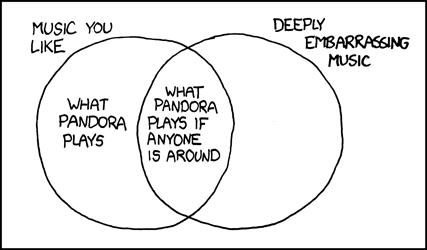
\includegraphics[width=4in]{pandora}
\end{center}

In both formal modeling and statistics classes, you will constantly
interact with concepts from basic probability theory.  In fact, many
game theory and statistics texts will include small amounts of
background information in passing.  This is often helpful, but can
lead some students to get confused about what distinguishes
statistical inference, the basic task in both statistics and game
theoretic models under uncertainty, from probability theory.  So
before you move forward into those areas of study, it is worth taking
some time to understand probability by itself.

The goal of inference is to take some observed data or known facts and
backwards induct something about the world.  For instance, we might want
to survey a random subset of American citizens and estimate the
average attitudes of the entire American electorate.  Alternatively, a
game theoretic model may require actors to estimate the location of
the median voter given the sequence of prior election outcomes
$x=(x_1, x_2, \ldots, x_n)$ and candidate positions $y=(y_1, y_2,
\ldots, y_n)$.

Probability theory is exactly the reverse.  Here we \textit{know} the
basic features of the data generating process (the parameters) and
want to understand what the data is likely to look like.  For
instance, we might have a fair coin and we want to understand the
likelihood of flipping 20 heads before the first tail shows up.
Obviously, most of the things you are going to be doing in graduate
school will be about inference.  Nonetheless, you \textit{really}
need to have a grasp of probability theory first.  

Probability is essentially thinking clearly about counting.  For the
simplest problems, all you need to know is the number of ways that some
set of outcomes $X$ could happen versus the total number of ways
things could have turned out.  So to begin with, you just need to
focus on getting a handle on the basic concepts of:
\bi
\item How to count events
\item How to think about and handle sets
\item How counting and sets relate to the concept of ``probability''
\item Conditional probability, independence, and Bayes' law
\ei

\newpage

\subsection{Counting rules}

\bi

\item {\bf Fundamental Theorem of Counting}: If there are $k$
  characteristics, each with $n_k$ alternatives, there are $\prod_{i =
    1}^k n_k$ possible outcomes.

\item We often need to count the number of ways to choose a subset
  from some set of possibilities.  The number of outcomes depends on
  two characteristics of the process: does the \emph{order} matter and
  is \emph{replacement} allowed?

\item If there are $n$ objects and we select $k < n$ of them, how many
  different outcomes are possible?  
\be
\item Ordered, with replacement: $n^k$
\item Ordered, without replacement: $ \frac{n!}{(n - k)!}$
\item Unordered, with replacement: $\frac{(n + k - 1)!}{(n - 1)! k!} =
  \left( \begin{array}{c}n + k - 1\\k \end{array}\right)$
\item Unordered, without replacement: ($n$ choose $k$):  $\frac{n!}{(n - k)! k!} =
  \left( \begin{array}{c}n \\k \end{array}\right)$ 


\ee 
\item Ordered events are sometimes referred to as permutations, while
  unordered events are combinations.  
\item In your introductory work, you will almost always be working
  with combinations.  
\ei

\subsection{Sets}

\bi
\item {\bf Set}: A set is any well defined collection of elements.  If
  $x$ is an element of $S$, $x \in S$.

\item Types of sets:
\be
\item Countably finite: a set with a finite number of elements, which
  can be mapped onto positive integers.\\ $S = \{1,2,3,4,5,6\}$
\item Countably infinite: a set with an infinite number of elements,
  which can still be mapped onto positive integers.\\ $S = \{1,
  \frac{1}{2}, \frac{1}{3}, \dots\}$
\item Uncountably infinite: a set with an infinite number of elements,
  which cannot be mapped onto positive integers. \\$S = \{x: x \in
  [0,1]\}$
\item Empty: a set with no elements.  \\$S = \{\emptyset\}$
\ee

\begin{center}
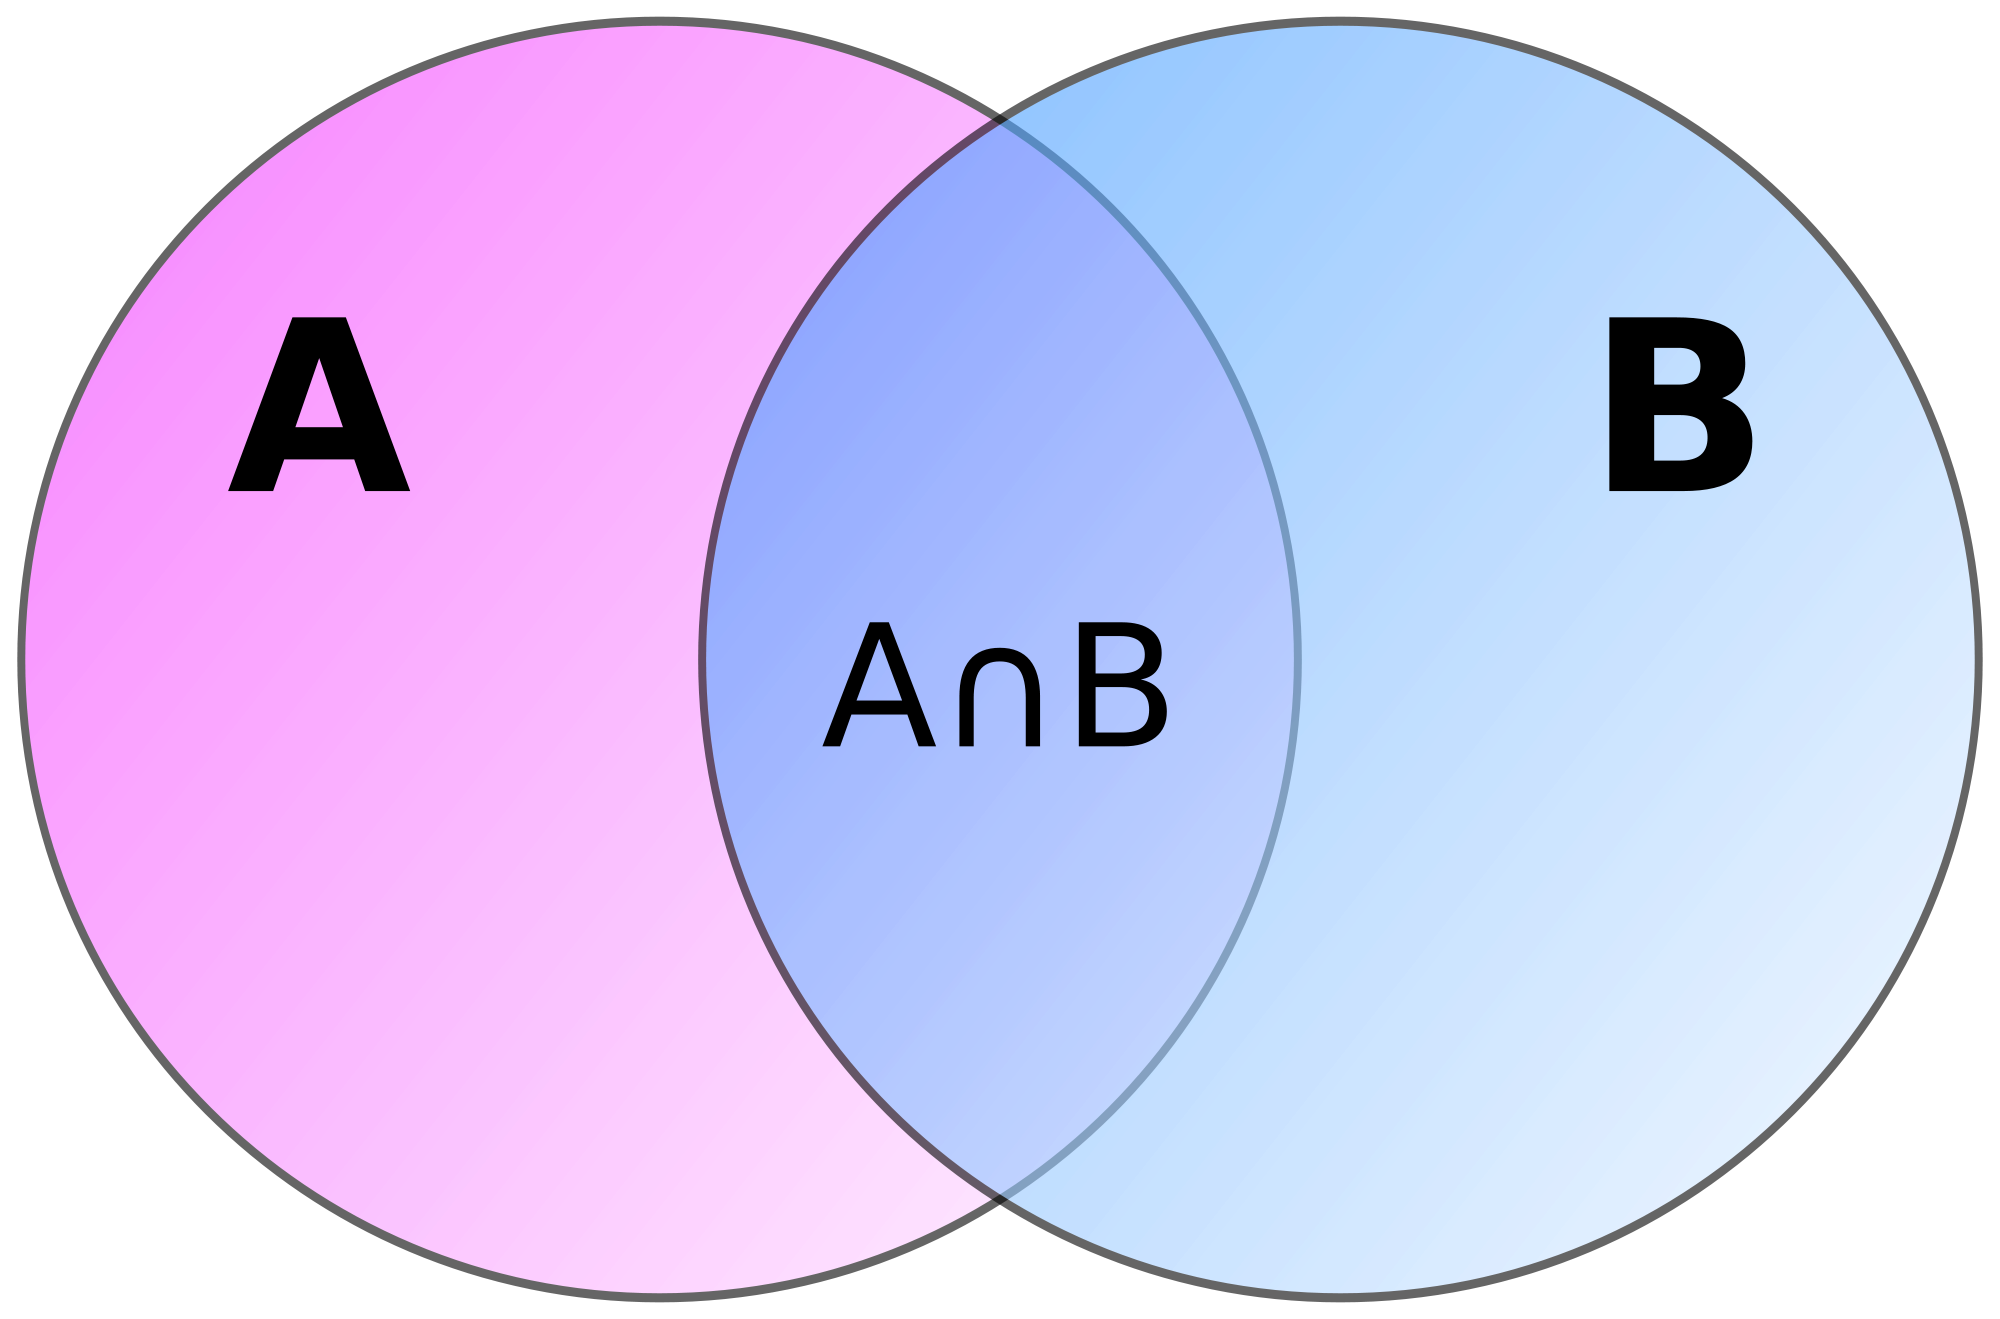
\includegraphics[width=2in]{Venn}
\end{center}


\item Set operations:
\be
\item {\bf Union}: The union of two sets $A$ and $B$, $A \cup B$, is
  the set containing all of the elements in $A$ or $B$.
\item {\bf Intersection}: The intersection of sets $A$ and $B$, $A
  \cap B$, is the set containing all of the elements in both $A$ and
  $B$.
\item {\bf Complement}: If set $A$ is a subset of $S$, then the
  complement of $A$, denoted $A^C$, is the set containing all of the
  elements in $S$ that are not in $A$.  \ee


\item Properties of set operations:\footnote{These are also
    \textit{very} important for understanding basic computer
    programming.}
\be
\item Commutative: $A \cup B = B \cup A$, $A \cap B = B \cap A$
\item Associative: $A \cup (B \cup C) = (A \cup B) \cup C$, $A \cap (B \cap C) = (A \cap B) \cap C$
\item Distributive: $A \cap (B \cup C) = (A \cap B) \cup (A \cap C)$,
  $A \cup (B \cap C) = (A \cup B) \cap (A \cup C)$
\item de Morgan's laws: $(A \cup B)^C = A^C \cap B^C$, $(A \cap B)^C = A^C \cup B^C$
\ee


\item {\bf Disjointness}: Sets are disjoint when they do not
  intersect, such that $A \cap B = \{\emptyset\}$.  A collection of
  sets is pairwise disjoint if, for all $i \neq j$, $A_i \cap A_j =
  \{\emptyset\}$.  A collection of sets form a partition of set $S$ if
  they are pairwise disjoint and they cover set $S$, such that
  $\bigcup_{i = 1}^k A_i = S$.  \ei


\subsection{Probability}
\bi

\item {\bf Probability}: Probability is an expression of uncertainty.
  Modern probability theory is a way of estimating our uncertainty
  about some future events given specific assumed properties of the
  world.  This is a formalization of basic human intuition about how
  to handle risk.  

\item {\bf Sample Space}: A set or collection of all possible outcomes
  from some process.  Outcomes in the set can be discrete elements
  (countable) or points along a continuous interval (uncountable).
\item Examples:
  \be
  \item Discrete:  the numbers on a die, the number of possible wars
        that could occur each year, whether a vote cast is republican
    or democrat.
  \item Continuous: GNP, arms spending, age.
  \ee

\item {\bf Probability Distribution/Function}: A probability \textit{function} on a
  sample space $S$ is a mapping $\Pr(A)$ from events in $S$ to the
  real numbers.  It is just like any other function.  We have some
  event/sample space $S$ we have a probability space (e.g., the
  probability of event $x$ happening is some number in $[0,1]$)and we have the
  function that translates $x$ into the probability space that we
  denote $p(x)$ or $f(x)$.  

\item {\bf Axioms of Probability}: Probability functions will satisfy
  the following three axioms (due to Kolmogorov). Define the number
  $\Pr(A)$ corresponding to each event $A$ in the sample space $S$ such
  that \be
  \item Axiom:  For any event $A$, $\Pr(A)\ge 0$.
  \item Axiom:  $\Pr(S)=1$
  \item Axiom: For any sequence of disjoint events
    $A_1,A_2,\ldots$ (of which there may be infinitely many),\\
    $\Pr\left( \bigcup\limits_{i=1}^k A_i\right)=\sum\limits_{i=1}^k
    \Pr(A_i)$ \ee



\item {\bf Example}: Let's say we are flipping two coins.  The sample
  space is $S={HH, HT, TH, TT}$.  


\begin{center}
\begin{tabular}{c | c}
\hline
Outcome & X=x \\
\hline
HH & 2 \\
HT & 1 \\
TH & 1 \\
TT & 0 \\
\hline
\end{tabular}
\end{center}

\begin{center}
\begin{tabular}{c | c}
\hline
x & p(x) \\
\hline
{TT} $\rightarrow$ 0 & .25 \\
{HT, TH} $\rightarrow$ 1 & .50 \\
{HH} $\rightarrow$ 2 & .25\\
\hline
Sum & 1.00 \\
\hline
\end{tabular}
\end{center}

\item {\bf Example}: Avoiding being a sure loser -- Axioms of probability and betting.
\be
\item A1: Rain and High above 68 degrees F tomorrow
\item A2: Rain and High at or below 68 degrees F tomorrow
\item A3: No Rain and High above 68 degrees F tomorrow
\item A4: No Rain and High at or below 68 degrees F tomorrow
\ee
\bi
\item These events are disjoint and exhaustive. 
\item Now specify prices for each event at which we are willing to sell or buy lottery tickets that pay \$1 if the event occurs
\item Define Pr(A1), Pr(A2), Pr(A3) and Pr(A4) as the prices you are willing to sell and buy at
\item What are the properties of these prices so that I can NOT make you are sure loser?
\ei
\be
\item No negative prices: Pr(E) $\geq 0$
\item What is the price for all events? Pr(All) $=1$
\item How about the Union of A1 and A2? Pr(A1 $\cup$ A2) = Pr(A1) + Pr(A2)
\ee

\item {\bf Basic Theorems of Probability}: Using these three axioms,
  we can define all of the common theorems of probability.  \be
  \item $\Pr(\emptyset)=0$
  \item $\Pr({A}^C)=1-\Pr(A)$
  \item For any event $A$, $0\le \Pr(A) \le 1$.
  \item If $A\subset B$, then $\Pr(A)\le \Pr(B)$.
  \item For any two events $A$ and $B$, $\Pr(A\cup
B)=\Pr(A)+\Pr(B)-\Pr(A\cap B)$
  \item For any sequence of $n$ events (which need not be disjoint)
$A_1,A_2,\ldots,A_n$,\\
$\Pr\left( \bigcup\limits_{i=1}^n
A_i\right) \leq \sum\limits_{i=1}^n \Pr(A_i)$
  \ee

\item Examples:  Let's assume we have an evenly-balanced, six-sided die.
Then,
  \be
  \item Sample space $S=\{ 1, 2, 3, 4, 5, 6 \}$
  \item $\Pr(1)=\cdots=\Pr(6)=1/6$
  \item $\Pr(\emptyset)=\Pr(7)=0$
  \item $\Pr\left( \{ 1, 3, 5 \} \right)=1/6+1/6+1/6=1/2$
  \item $\Pr\left( \ol{\{ 1, 2 \}} \right)= \Pr\left( \{ 3, 4, 5, 6 \}
  \right) = 2/3$
  \item Let $B=S$ and $A=\{ 1,2,3,4,5 \}\subset B$.  Then
$\Pr(A)=5/6<\Pr(B)=1$.
  \item Let $A=\{ 1, 2, 3 \}$ and $B=\{ 2, 4, 6 \}$.  Then $A\cup B=\{
1, 2, 3, 4, 6\}$, $A\cap B=\{2\}$, and
  \beqa
  \Pr(A\cup B)&=&\Pr(A)+\Pr(B)-\Pr(A\cap B)\non\\
              &=& 3/6  + 3/6  - 1/6\non\\
              &=& 5/6\non
  \eeqa
  \ee
\ei

\subsection{Conditional Probability and Bayes' Law}
\bi

\item {\bf Conditional Probability}:  The conditional probability
$\Pr(A|B)$ of an event $A$ is the probability
of $A$, given that another event $B$ has occurred.  It is calculated as
$$\Pr(A|B)=\frac{\Pr(A\cap B)}{\Pr(B)}$$



\item Example:  Assume $A$ and $B$ occur with the following frequencies: $\quad$
\begin{tabular}{lcc}
         & $A$          & $\ol{A}$ \\\hline
$B$      & $n_{ab}$     & $n_{\ol{a}b}$ \\
$\ol{B}$ & $n_{a\ol{b}}$ & $n_{\ol{ab}}$
\end{tabular}\\
and let $n_{ab}+n_{\ol{a}b}+n_{a\ol{b}}+n_{\ol{ab}}=N$.  Then
  \be
  \item $\Pr(A)\approx\frac{n_{ab}+n_{a\ol{b}}}{N}$
  \item $\Pr(B)\approx\frac{n_{ab}+n_{\ol{a}b}}{N}$
  \item $\Pr(A\cap B)\approx\frac{n_{ab}}{N}$
  \item $\Pr(A|B)\approx\frac{\Pr(A\cap B)}{\Pr(B)}=
         \frac{n_{ab}}{n_{ab}+n_{\ol{a}b}}$
  \item $\Pr(B|A)\approx\frac{\Pr(A\cap B)}{\Pr(A)}=
         \frac{n_{ab}}{n_{ab}+n_{a\ol{b}}}$
  \ee

\item Example:  A six-sided die is rolled.  What is the probability of a
1, given the outcome is an odd number?  Let $A=\{ 1 \}$, $B=\{ 1, 3, 5
\}$, and $A\cap B=\{ 1 \}$.  Then, $\Pr(A|B)=\frac{\Pr(A\cap
B)}{\Pr(B)}=\frac{1/6}{1/2}=1/3$.

\item {\bf Multiplicative Law of Probability}: The probability of the
intersection of two events $A$ and $B$ is $$\Pr(A\cap
B)=\Pr(A)\Pr(B|A)=\Pr(B)\Pr(A|B)$$ which follows directly from the
definition of conditional probability.

\item {\bf Law of Total Probability}:  Let $S$ be the sample space of
some experiment and let the disjoint $k$ events $B_1,\ldots,B_k$
partition $S$.  If $A$ is some other event in $S$, then the events
$AB_1, AB_2, \ldots, AB_k$ will form a partition of $A$ and we can write
$A$ as $$A=(AB_1)\cup\cdots\cup (AB_k)$$  Since the $k$ events are
disjoint,
\beqa
\Pr(A)&=&\sum\limits_{i=1}^k \Pr(A,B_i)\non\\
      &=&\sum\limits_{i=1}^k \Pr(B_i)\Pr(A|B_i)\non
\eeqa
Sometimes it is easier to calculate the conditional probabilities and
sum them than it is to calculate $\Pr(A)$ directly.

\subsection{Bayesian thinking}

\item {\bf Bayes Rule}: Assume that events $B_1,\ldots,B_k$ form a
partition of the space $S$.  Then $$\Pr(B_j|A)= \frac{\Pr(A, B_j)}
{\Pr(A)} = \frac{\Pr(B_j)
\Pr(A|B_j)}{\sum\limits_{i=1}^k \Pr(B_i)\Pr(A|B_i)}$$
If there are only two states of $B$, then this is just
$$\Pr(B_1|A)=\frac{\Pr(B_1)\Pr(A|B_1)}
{\Pr(B_1)\Pr(A|B_1)+\Pr(B_2)\Pr(A|B_2)}$$


\item If this was a continuous distribution we could write this as:

$$\Pr(B_j|A)= \frac{\Pr(A, B_j)}
{\Pr(A)} = \frac{\Pr(B)
\Pr(A|B)}{\lint\limits_{\infty}^\infty \Pr(A, B)\Pr(B)}$$


\item Bayes rule  determines the posterior probability of a state or
type  $\Pr(B_j|A)$ by calculating the probability $\Pr(A B_j)$ that both
the event $A$ and the state $B_j$ will occur and dividing it by the
probability that the event will occur regardless of the state (by
summing across all $B_i$).

\item  Often Bayes' rule is used when one wants to calculate a posterior
probability about the ``state" or type of an object, given that some
event has occurred.  The states could be something like
Normal/Defective, Normal/Diseased, Democrat/Republican, etc.  The event
on which one conditions could be something like a sampling from a batch
of components, a test for a disease, or a question about a policy
position.

\item {\bf Prior and Posterior Probabilities}:  In the above, $\Pr(B_1)$
is often called the prior probability, since it's the probability of
$B_1$ before anything else is known.  $\Pr(B_1|A)$ is called the
posterior probability, since it's the probability after other
information is taken into account.

\item Examples:
  \be
  \item A test for cancer correctly detects it 90\%  of the time, but
incorrectly identifies a person as having cancer 10\% of the time.  If
10\% of all people have cancer at any given time, what is the
probability that a person who tests positive actually has cancer?\\[6pt]


  \item In Boston, 30\% of the people are conservatives, 50\% are
liberals, and 20\% are independents.  In the last election, 65\% of
conservatives, 82\% of liberals, and 50\% of independents voted.  If a
person in Boston is selected at random and we learn that s/he did not
vote last election, what is the probability s/he is a liberal?\\[6pt]
  \ee

\ei

\subsection{Independence}

\bi

\item {\bf Independence}:  If the occurrence or nonoccurrence of either
events $A$ and $B$ have no effect on the occurrence or nonoccurrence of
the other, then $A$ and $B$ are independent.  If $A$ and $B$ are
independent, then
  \be
  \item $\Pr(A|B)=\Pr(A)$
  \item $\Pr(B|A)=\Pr(B)$
  \item $\Pr(A\cap B)=\Pr(A)\Pr(B)$
  \ee

\item {\bf Pairwise independence}: A set of more than two events $A_1,
  A_2, \dots, A_k$ is pairwise independent if $\Pr(A_i\cap
  A_j)=\Pr(A_i)\Pr(A_j)$, $\forall i\neq j$.  Note that this does
  \emph{not} necessarily imply that $\Pr(\bigcap_{i=1}^k A_i) =
  \prod_{i = 1}^K \Pr(A_i)$.

\item{\bf Conditional independence}: If the occurrence of $A$ or $B$
  conveys no information about the occurrence of the other, once you
  know the occurrence of a third event $C$, then $A$ and $B$ are
  conditionally independent (conditional on $C$): \be
  \item $\Pr(A|B \cap C)=\Pr(A|C)$
  \item $\Pr(B|A \cap C)=\Pr(B|C)$
  \item $\Pr(A\cap B|C)=\Pr(A|C)\Pr(B|C)$
\ee

\item Conditional independence is one of the fundamental assumptions
  deployed for most statistical estimation techniques.  It is a
  \textit{very} strong assumption.   

\ei


\section{Random variables}

\begin{center}
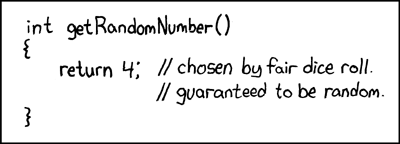
\includegraphics[width=4in]{randomnumber}
\end{center}

The intellectual beginnings of probability began in gambling, and this
is still the easiest way to teach it.  In probability theory, random
variables are something abstract.  A random variable is a yet-to-be
observed value.  What is the probability that a coin will turn up
heads?  What is the probability the next card will be an ace?

Depending on the kinds of events we are talking about, we have
identified several ``types'' of random variables.  These variables
have known functional forms.  Moreover, these functions have been
extensively studied and their properties are well understood.  The
focus of this last section of lecturing is to get you familiar with
these ``kinds'' of variables.  

Don't obsess about memorizing any of this.  You will never be that far
from Wikipedia.  Focus on understanding:
\bi
\item How this part of the lectures relates to the previous half of
  lectures
\item Get a handle for the basic mapping of data types and the random
  variable ``types'' they go with (e.g., coin flips $\rightarrow$
  binomial).
\item The basic properties of random variables we care about (e.g.,
  expected values, etc.)
\ei


\subsection{Levels of Measurement}

\bi

\item In empirical research, data can be classified along several
  dimensions.  We have already distinguished between discrete
  (countable) and continuous (uncountable) data.  We can also look at
  the precision with which the underlying quantities are measured.

\item {\bf Nominal}: Discrete data are nominal if there is no way to
  put the categories represented by the data into a meaningful order.
  Typically, this kind of data represents names (hence `nominal') or
  attributes, like Republican or Democrat.

\item {\bf Ordinal}: Discrete data are ordinal if there is a logical
  order to the categories represented by the data, but there is no
  common scale for differences between adjacent categories.  Party
  identification is often measured as ordinal data.

\item {\bf Interval}: Discrete or continuous data are interval if
  there is an order to the values and there is a common scale, so that
  differences between two values have substantive meanings.  Dates are
  an example of interval data.

\item {\bf Ratio}: Discrete or continuous data are ratio if the data
  have the characteristics of interval data and zero is a meaningful
  quantity.  This allows us to consider the ratio of two values as
  well as difference between them.  Quantities measured in dollars,
  such as per capita GDP, are ratio data.

\ei


\subsection{Discrete Distributions}
\bi

\item {\bf Random Variable}: A random variable is a real-valued function
defined on the sample space $S$; it assigns a real number to every outcome $s \in S$.

\item {\bf Discrete Random Variable}: $Y$ is a discrete random variable
if it can assume only a finite or countably infinite number of distinct
values.

\item Examples:  number of wars per year, heads or tails, voting
Republican or Democrat, number on a rolled die.

\item {\bf Probability Mass Function}: For a discrete random variable
$Y$, the probability mass function (pmf)\footnote{Also referred to
simply as the ``probability distribution."}
$p(y)=\Pr(Y=y)$ assigns probabilities to a countable number of
distinct $y$ values such that
  \be
  \item $0\le p(y)\le 1$
  \item $\sum\limits_y p(y)=1$
  \ee

\item {\bf Example}: For one fair six-sided die, there is an equal
probability of rolling any number.  Since there are six sides, the
probability mass function is then $p(y)=1/6$ for $y=1,\ldots,6$.  Each
$p(y)$ is between 0 and 1.  And, the sum of the $p(y)$'s is 1.  If
there are two six-sided dice, the probability mass function is shown
below.  

\begin{center}
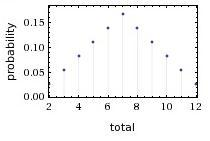
\includegraphics[width=3in]{TwoDie2}
\end{center}



\item {\bf Cumulative Distribution}:  The cumulative distribution $F(y)$
or $\Pr(Y\le y)$ is the probability that $Y$ is less than or equal to
some value $y$, or $$\Pr(Y\le y)=\sum\limits_{i\le y} p(i)$$.  The CDF must satisfy these properties:
\be
\item $F(y)$ is non-decreasing in $y$.
\item $\lim_{y \to -\infty} F(y) = 0$ and $\lim_{y \to \infty} F(y) = 1$
\item $F(y)$ is right-continuous.
\ee
\item \parbox[t]{4.5in}{Example:  For a fair die, $\Pr(Y\le 1)=1/6$, $\Pr(Y\le
3)=1/2$, and $\Pr(Y\le 6)=1$.}\parbox{1.5in}{}
\ei

\begin{center}
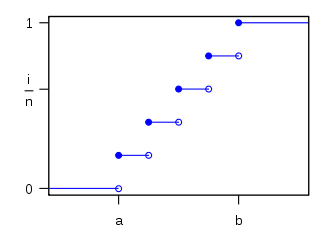
\includegraphics[width=3in]{CDFDIE}
\end{center}


\subsection{Continuous Distributions}
\bi

\item {\bf Continuous Random Variable}:  $Y$ is a continuous random
variable if there exists a nonnegative function $f(y)$ defined for all
real $y\in (-\infty,\infty)$, such that for any interval $A$, $$\Pr(Y\in
A)=\lint_A f(y)dy$$

\item Examples: age, income, GNP, temperature

\item {\bf Probability Density Function}:  The function $f$ above is
called the probability density function (pdf) of $Y$ and must satisfy
  \be
  \item $f(y)\ge 0$
  \item $\lint_{-\infty}^\infty f(y)dy=1$
  \ee
Note also that $\Pr(Y=y)=0$ --- i.e., the probability of any point $y$ is
zero.

\item \textbf{Example}: Uniform distribution (e.g., $f(x) = 1$). 

$$ f(x)=\begin{cases}
  \frac{1}{b - a} & \mathrm{for}\ a \le x \le b, \\
  0 & \mathrm{for}\ x<a\ \mathrm{or}\ x>b
  \end{cases} $$

\begin{center}
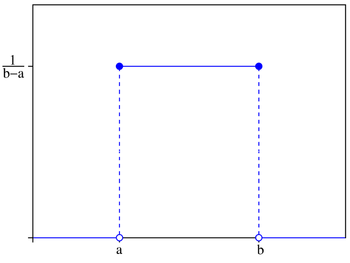
\includegraphics[width=3in]{UniformPdf}
\end{center}


\item {\bf Cumulative Distribution}: Because the probability that a
  continuous random variable will assume any particular value is zero,
  we can only make statements about the probability of a continuous
  random variable being within an interval.  The cumulative
  distribution gives the probability that $Y$ lies on the interval
  $(-\infty,y)$ and is
  defined as $$F(y)=\Pr(Y\le y)=\lint_{-\infty}^y f(s)ds$$  Note that
  $F(y)$ has similar properties with continuous distributions as it
  does with discrete - non-decreasing, continuous (not just
  right-continuous), and $\lim_{y \to -\infty} F(y) = 0$ and $\lim_{y
    \to \infty} F(y) = 1$.



  Similarly, we can also make probability statements about $Y$ falling
  in an interval $a\le y\le b$. $$\Pr(a\le y\le b)=\lint_a^b f(y)dy$$

\item Example: $f(y)=1, \quad 0<y<1$.  Find $F(y)$ and
$\Pr(.5<y<.75)$. $$F(y)=\lint_0^y f(s)ds = \int_0^y 1 ds = \left. s
\right|_0^y = y$$ $$\Pr(.5<y<.75)= \int_{.5}^{.75} 1 ds = \left. s
\right|_{.5}^{.75} = .25$$ 
\parbox{1.5in}



\begin{center}
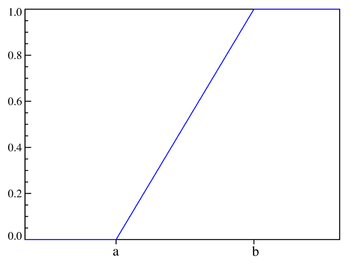
\includegraphics[width=3in]{UniformCDF}
\end{center}


\item $F'(y)=\frac{dF(y)}{dy}=f(y)$

\ei

\subsection{Joint Distributions}

\bi
\item Often, we are interested in two or more random variables defined
  on the same sample space.  The distribution of these variables is
  called a joint distribution.  Joint distributions can be made up of
  any combination of discrete and continuous random variables.
\item Example: Suppose we are interested in the outcomes of flipping a
  coin and rolling a 6-sided die at the same time.  The sample space
  for this process contains 12 elements: $$\{h1, h2, h3, h4, h5, h6,
  t1, t2, t3, t4, t5, t6\}$$ We can define two random variables $X$
  and $Y$ such that $X = 1$ if heads and $X = 0$ if tails, while $Y$
  equals the number on the die.  We can then make statements about the
  joint distribution of $X$ and $Y$.
\item {\bf Joint discrete random variables}: If both $X$ and $Y$ are
  discrete, their joint probability mass function assigns
  probabilities to each pair of outcomes
$$ p(x, y) = \Pr(X = x, Y = y)$$
Again, $p(x,y) \in [0,1]$ and $\sum\sum p(x,y) = 1$.

If we are interested in the marginal probability of one of the two
variables (ignoring information about the other variable), we can
obtain the marginal pmf by summing across the variable that we don't
care about:
$$p_X(x) = \sum_i p(x, y_i)$$

We can also calculate the conditional pmf for one variable, holding
the other variable fixed.  Recalling from the previous lecture that
$\Pr(A|B)=\frac{\Pr(A\cap B)}{\Pr(B)}$, we can write the conditional
pmf as
$$ p_{Y|X}(y|x) = \frac{p(x,y)}{p_X(x)}, \quad p_X(x) > 0$$

\item {\bf Joint continuous random variables}: If both $X$ and $Y$ are
  continuous, their joint probability density function defines their
  distribution:
$$ \Pr((X,Y) \in A) = \int\!\!\!\int_A f(x,y)dx dy$$
Likewise,   $f(x,y)\ge 0$ and $\int_{-\infty}^\infty\int_{-\infty}^\infty f(x,y)dxdy =1 $.

Instead of summing, we obtain the marginal probability density
function by integrating out one of the variables:

$$f_X(x) = \int_{-\infty}^\infty f(x,y)dy $$

Finally, we can write the conditional pdf as

$$ f_{Y|X}(y|x) = \frac{f(x,y)}{f_X(x)},\quad f_X(x) > 0$$

\ei

\subsection{Expectation}
\bi

\item We often want to summarize some characteristics of the
  distribution of a random variable.  The most important summary is
  the expectation (or expected value, or mean), in which the possible
  values of a random variable are weighted by their probabilities.

\item {\bf Expectation of Discrete Random Variable}:  The expected value
of a discrete random variable $Y$ is $$E(Y)=\sum\limits_{y} y p(y)$$  In
words, it is the weighted average of the possible values $y$ can take
on, weighted by the probability that $y$ occurs.  It is not necessarily
the number we would expect $Y$ to take on, but the average value of $Y$
after a large number of repetitions of an experiment.

\item Example: For a fair die, $$E(Y)=\sum\limits_{y=1}^6 y
p(y)=\frac{1}{6}\sum\limits_{y=1}^6 y = 7/2$$  We would never expect the
result of a rolled die to be $7/2$, but that would be the average over a
large number of rolls of the die.

\item {\bf Expectation of a Continuous Random Variable}:  The expected
value of a continuous random variable is similar in concept to that of
the discrete random variable, except that instead of summing using
probabilities as weights, we integrate using the density to weight.
Hence, the expected value of the continuous variable $Y$ is defined by
$$E(Y)=\lint_{-\infty}^\infty y f(y) dy$$

\item Example:  Find $E(Y)$ for $f(y)=\frac{1}{1.5}, \quad 0<y<1.5$.
$$E(Y)=\lint_0^{1.5} \frac{1}{1.5} y dy= \left. \frac{1}{3} y^2
\right|_0^{1.5} = .75$$

\item {\bf Expected Value of a Function}:
  \be
  \item \pbof{Discrete:}   $E[g(Y)]=\sum\limits_y g(y)p(y)$
  \item \pbof{Continuous:} $E[g(Y)]=\lint_{-\infty}^\infty
g(y)f(y)dy$
  \ee

\item {\bf Other Properties of Expected Values}:
  \be
  \item $E(c)=c$
  \item $E[E[Y]] = E[Y]$ (because the expected value of a random variable is a constant)
  \item $E[c g(Y)]= c E[g(Y)]$
  \item $E[g(Y_1) + \cdots + g(Y_n)]=E[g(Y_1)]+\cdots+E[g(Y_n)]$
  \ee

\item {\bf Variance}:  We can also look at other summaries of the
distribution, which build on the idea of taking expectations.
Variance tells us about the ``spread" of the distribution; it is the
expected value of the squared deviations from the mean of the
distribution.  The standard deviation is simply the square root of the
variance.
  \be
  \item \pbof{Variance:} $\sigma^2= \Var(Y) = E[(Y - E(Y))^2] =  E(Y^2)-[E(Y)]^2$
  \item \pbof{Standard Deviation:} $\sigma= \sqrt{\Var(Y)}$
  \ee

\item {\bf Covariance and Correlation}: The covariance measures the
  degree to which two random variables vary together; if the
  covariance is positive, X tends to be larger than its mean when Y is
  larger than its mean.  The covariance of a variable with itself is
  the variance of that variable.

$$\Cov(X,Y) = E[(X - E(X))(Y - E(Y))] = E(XY) - E(X)E(Y)$$

The correlation coefficient is the covariance divided by the standard
deviations of X and Y.  It is a unitless measure and always takes on
values in the interval $[-1,1]$.

$$\rho = \frac{\Cov(X,Y)}{\sqrt{\Var(X)\Var(Y)}} = \frac{\Cov(X,Y)}{\SD(X)\SD(Y)}$$


\item {\bf Conditional Expectation}: With joint distributions, we are
  often interested in the expected value of a variable $Y$ if we could
  hold the other variable $X$ fixed.  This is the conditional
  expectation of $Y$ given $X = x$: \be
\item $Y$ discrete:  $E(Y|X = x) = \sum_y yp_{Y|X}(y|x)$
\item $Y$ continuous: $E(Y|X = x) = \int_y yf_{Y|X}(y|x)dy$ \ee The
  conditional expectation is often used for prediction when one knows
  the value of $X$ but not $Y$; the realized value of $X$ contains
  information about the unknown $Y$ so long as $E(Y|X = x) \neq E(Y)
  \forall x$.


\ei


\subsection{Special Discrete Distributions}
\bi

\item {\bf Binomial Distribution}: $Y$ is distributed binomial if it
represents the number of ``successes" observed in $n$ independent,
identical ``trials," where the probability of success in any trial is
$p$ and the probability of failure is $q=1-p$.\\[6pt]
For any particular sequence of $y$ successes and $n-y$ failures,
the probability of obtaining that sequence is $p^y q^{n-y}$ (by the
multiplicative law and independence).  However, there are
$\binom{n}{y}=\frac{n!}{(n-y)!y!}$ ways of obtaining a sequence with $y$
successes and $n-y$ failures.  So the binomial distribution is given by
$$p(y)=\binom{n}{y}p^y q^{n-y}, \quad y=0,1,2,\ldots,n$$ with mean
$\mu=E(Y)=np$ and variance $\sigma^2=V(Y)=npq$.

\item Example: Republicans vote for Democrat-sponsored bills 2\% of the time.
What is the probability that out of 10 Republicans questioned, half
voted for a particular Democrat-sponsored bill?  What is the mean number
of Republicans voting for Democrat-sponsored bills?  The variance?
  \be
  \item \parbox[t]{4.25in}{$p(5)=\binom{10}{5}(.02)^5 (.98)^5=.073$}
  \parbox{1.5in}{\hfill {}}
  \item $E(Y)=np=10(.02)=.2$
  \item $V(Y)=npq=10(.02)(.98)=.196$
  \ee
\item {\bf Poisson Distribution}:  A random variable $Y$ has a Poisson
distribution if $$p(y)=\frac{\lambda^y}{y!}e^{-\lambda}, \quad
y=0,1,2,\ldots, \quad \lambda>0$$  The Poisson has the unusual feature
that its expectation equals its variance: $E(Y)=V(Y)=\lambda$.
The Poisson distribution is often used to model event counts:  counts of
the number of events that occur during some unit of time.  $\lambda$ is
often called the ``arrival rate."

\item \parbox[t]{4.5in}{Example: Border disputes occur between two
countries at a rate of 2 per month.  What is the probability of 0, 2,
and less than 5 disputes occurring in a month?}
\parbox{1.5in}{\hfill {}}
  \be
  \item $p(0)=\frac{2^0}{0!}e^{-2}=.13$
  \item $p(2)=\frac{2^2}{2!}e^{-2}=.27$
  \item $\Pr(Y<5)=\sum\limits_{y=0}^4 \frac{2^y}{y!}e^{-2}= .95$
  \ee
\ei

\subsection{Special Continuous Distributions}
\bi

\item {\bf Uniform Distribution}:  A random variable $Y$ has a
continuous uniform distribution on the interval $(\alpha,\beta)$ if its
density is given by $$f(y)=\frac{1}{\beta-\alpha}, \quad \alpha\le y\le
\beta$$  The mean and variance of $Y$ are $E(Y)=\frac{\alpha+\beta}{2}$
and $V(Y)=\frac{(\beta-\alpha)^2}{12}$.

\item \parbox[t]{4.5in}{Example: $Y$ uniformly distributed over $(1,3)$.}
\parbox{1.5in}{\hfill {}}

\item {\bf Normal Distribution}:  A random variable $Y$ is normally
distributed with mean $E(Y)=\mu$ and variance $V(Y)=\sigma^2$ if its
density is
$$f(y)=\frac{1}{\sqrt{2\pi}\sigma}e^{-\frac{(y-\mu)^2}{2\sigma^2}}$$

\item \parbox[t]{4.5in}{Example: $Y$ normally distributed with mean
$\mu=0$ and variance $\sigma^2=.1$}
\parbox{1.5in}{\hfill {}}

\ei

\subsection{Summarizing Observed Data}

\bi

\item So far, we've talked about distributions in a theoretical sense,
  looking at different properties of random variables.  We don't
  observe random variables; we observe realizations of the random
  variable.

\item {\bf Central tendency}: The central tendency describes the
  location of the ``middle'' of the observed data along some scale.
  There are several measures of central tendency.  \be
\item {\bf Sample mean}: This is the most common measure of central
  tendency, calculated by summing across the observations and dividing
  by the number of observations.
$$ \bar{x} = \frac{1}{n}\sum_{i=1}^{n}x_i$$
The sample mean is an estimate of the expected value of a
distribution.

\item {\bf Sample median}: The median is the value of the ``middle''
  observation.  It is obtained by ordering $n$ data points from
  smallest to largest and taking the value of the $n+1/2$th
  observation (if $n$ is odd) or the mean of the $n/2$th and
  $(n/2)+1$th observations (if $n$ is even).

\item {\bf Sample mode}: The mode is the most frequently observed value in the data:
$$m_x = X_i : n(X_i) > n(X_j) \forall j\neq i$$
When the data are realizations of a continuous random variable, it
often makes sense to group the data into bins, either by rounding or
some other process, in order to get a reasonable estimate of the mode.

\item Exercise: Calculate the sample mean, median, and mode for the
  following two variables, X and Y.
\begin{center}
\begin{tabular}{|l|cccccccccc|}
\hline
X & 6 & 3 & 7 & 5 & 5 & 5 & 6 & 4 & 7 & 2\\
\hline
Y & 1 & 2 & 1 & 2 & 2 & 1 & 2 & 0 & 2 & 0\\
\hline
\end{tabular}
\end{center}
\ee 

\item {\bf Dispersion}: We also typically want to know how spread out
  the data are relative to the center of the observed distribution.
  Again, there are several ways to measure dispersion.  \be

\item {\bf Sample variance}: The sample variance is the sum of the
  squared deviations from the sample mean, divided by the number of
  observations minus 1.

$$ \Var(X) = \frac{1}{n-1}\sum_{i = 1}^n (x_i - \bar{x})^2$$

Again, this is an estimate of the variance of a random variable; we
divide by $n - 1$ instead of $n$ in order to get an unbiased estimate.

\item {\bf Standard deviation}: The sample standard deviation is the
  square root of the sample variance.

$$ \SD(X) = \sqrt{\Var(X)} = \sqrt{\frac{1}{n-1}\sum_{i = 1}^n (x_i - \bar{x})^2}$$

\item {\bf Median absolute deviation (MAD)}: The MAD is a different
  measure of dispersion, based on deviations from the median rather
  than deviations from the mean.

$$MAD(X) = median(|x_i - median(x)|)$$

\item Exercise:  Calculate the sample variance, standard deviation, and MAD for the following two variables, X and Y.
\begin{center}
\begin{tabular}{|l|cccccccccc|}
\hline
X & 6 & 3 & 7 & 5 & 5 & 5 & 6 & 4 & 7 & 2\\
\hline
Y & 1 & 2 & 1 & 2 & 2 & 1 & 2 & 0 & 2 & 0\\
\hline
\end{tabular}
\end{center}
\ee

\item {\bf Covariance and Correlation}: Both of these quantities measure the degree to which two variables vary together, and are estimates of the covariance and correlation of two random variables as defined above.

\be

\item {\bf Sample covariance}: $\Cov(X,Y) = \frac{1}{n-1}\sum_{i = 1}^n(x_i - \bar{x})(y_i - \bar{y})$

\item {\bf Sample correlation}: $r = \frac{\Cov(X,Y)}{\sqrt{\Var(X)\Var(Y)}}$

\item Exercise:  Calculate the sample covariance and correlation coefficient for the following two variables, X and Y.
\begin{center}
\begin{tabular}{|l|cccccccccc|}
\hline
X & 6 & 3 & 7 & 5 & 5 & 5 & 6 & 4 & 7 & 2\\
\hline
Y & 1 & 2 & 1 & 2 & 2 & 1 & 2 & 0 & 2 & 0\\
\hline
\end{tabular}
\end{center}
\ee

\ei



\end{document}